\chapter{Linear Projection}
\label{chapter:projection}

We would like to define a region of interest that contains only one uni-model for exploitation.
Also, some algorithms, e.g. SPSO, requires a well-defined hypercube search space with fixed-value constraints in each dimension.
Defining the projection onto subspace can be described as a model selection.
In our case, this process does not require high accuracy, yet has a strict demand on time consumption.
Combining the requirements, we use a linear projection matrix to project the original search space 
onto a subspace with feasible solutions bounded within $[0,1]$ in each dimension.

One of the advantage for using projection matrix is that for a problem with $\ell$ variables, 
a linear projection matrix on homogeneous coordinate only requires $(\ell+1)^2$ hyperparameters to be optimized.
Therefore, less hyperparameters are assigned than directly define each hyperplane borders or vertices.  
This reduces the parameters that we need to optimize and results in less time consumption during model selection.
We also use the (1+1)-Evolutionary Strategy ((1+1)-ES) to optimize the matrix.
The (1+1)-ES is a fast and simple evolutionary strategy,
that allows us to rapidly approximate a high dimensional projection matrix within given number of iterations.

Furthermore, subspace projection also gives advantage for solving \textit{inseparable problems}.
For variabels that are not independent, projection allows the algorithm
to solve an easier, rotated and sheared problem on subspace, as shown in Figure~\ref{fig:Projected_ROI}.
The homogeneous projection matrix seperates the original ROI into less overlapped ROI, 
which reduces redundant search and sometimes enlarges the crutial regions.

In the following sections, we first describe the cannonical affine transformation.
Then we discuss how the projection matrix allows linear projection in a homogeneous coordinate.
Finally, we give details of how we design the cost function and how we utilize the (1+1)-ES to optimize the projection matrix.

\begin{figure}
\centering
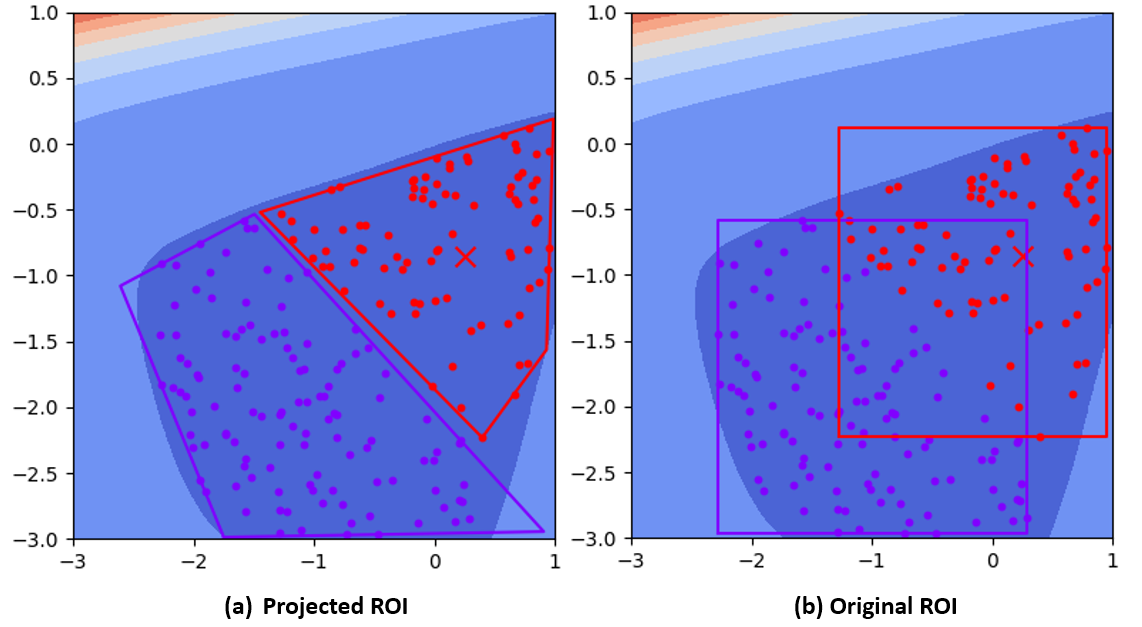
\includegraphics[width=\textwidth]{Projected_ROI}
\caption{Projecting inseparable problems onto subspace.}\label{fig:Projected_ROI}
\end{figure}



\section{Affine Transformation}
In geometry, an affine transformation preserves points, straight lines and planes.
For two affine spaces $A$ and $B$ and any pair of points $P, Q \in A$,
an affine transformation $f$ determines a linear transformation $\varphi$ that can formally defined as:
\begin{displaymath}
\overrightarrow{f(P)f(Q)} = \varphi \overrightarrow{(PQ)}
\end{displaymath}

\subsection{Translation}
\subsection{Rotation}
\subsection{Scaling}
\subsection{Shear}
\subsection{Affine transformation matrix}






\section{Projection}

\subsection{Basic Projection}


\subsection{Homogeneous Coordinate}
Augmented Matrix



\subsection{Perspective Projection}





\section{Optimization for Projection Matrix}

After identifying different clusters of samples, which represents a uni-modal, 
we would like to further define a reasonably good ROI.
In order to obtain a nice ROI for a problem with $D$ variables, 
we need to optimize the $(D+1)^2$ parameters in the projection matrix with a loss function.
The loss function should cost little computational time and should suggest the right direction for optimization, 
in order to match the restrictions of a well-defined ROI.
Also, the optimization only needs to define a reasonably well ROI for the alogirthms to search.  
In the later iterations, the matrix update procedure allows us to define a more accurate ROI with a better insight of the uni-modal subproblem.
In our case, it is acceptable to sacrefice a bit of accuracy for computational time in hyperparameters tuning.  
We will describe the desgin of our loss function and the advantage of using a (1+1)-ES to optimize the matrix in the following sections.  


\subsection{Loss function}

The goal of the ROI is to seperate the search space into non-overlapping subspaces, 
each containing an approximately normalized fitness hill.
Therefore, we would like to keep all the particles that belong to this cluster in the boundary $[0,1]^D$, 
while excluding all the particles that belong to other clusters.
We would also like each underlying model for each subproblem to be a multivariate gaussian distribution with mean around the center $[0.5]^D$
and the covariance matrix to be approximately $0.2I$, where $I$ is an identicle matrix.
Finally, since the we project the particle positions in a homogeneous coordinate, 
the correlations between reconstructed positions on the subspace might not be identicle to the original ones.
We would like to minimize the transformation error.

In our loss function, we considered the following features:
\begin{itemize}
    \item Distances to the boundary for the \textbf{points within the cluster} yet excluded in the ROI.
    \item Distances to the boundary for the \textbf{points of other clusters} yet included in the ROI.
    \item Distance of the weighted \textbf{mean} to the center of subspace $[0.5]^D$
    \item The Mean Absolute Error (MAE) for each element in the weighted \textbf{covariance matrix} to a scaled identicle matrix
    \item The sum of \textbf{reconstruction} error for each particle 
\end{itemize} 

For a possible solution of the projection matrix $X = [x_1, x_2, ..., x_{(d+1)^2}]$ of a problem with $d$ variables, 
we define the loss function $f$ as: 
\begin{equation} 
f(X) = D_should_be_in + D_should_be_out + D_center + MSE_covariance + 
\end{equation}


\subsection{Optimization Algorithms}

Describe the difficulty of finding a fast yet powerful algorithm for \textit{hyperparameters optimization}.

Initialize with a translation + scaling matrix.

We first tried CMA-ES.

Later, we utilize the (1+1)-ES, described in Algorithm~\ref{algo:1+1ES}.


